If the \textcolor{blue}{$sub$-$trip$} starts from the first stop,
the success rate drops significantly (and becomes unpredictable) due to
the reason illustrated in the following picture: \\

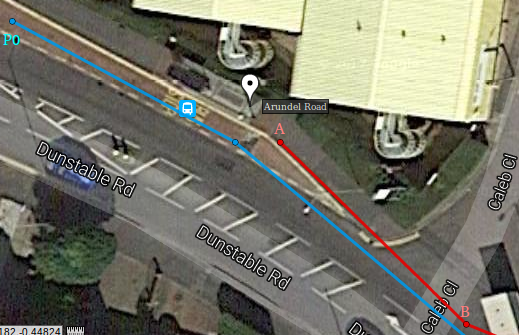
\includegraphics[scale = 0.7]{figs/stop0.png} \\

One can see that $err(P_0, S_{P_0}) = \frac{|{P_0}A| + |{P_0}B|}{|AB|} - 1$
might become large. In fact, accumulated errors for the first
few points (when the bus is not on any route yet) are so large the total
sum exceeds $n\epsilon$ even if errors for the next points are small. \\

The conclusion is thus to discard the first few GPS points and start using
$FollowsPath$ predicate after the bus has moved for a while and is following
some route.
